\chapter{Resultados}

Neste capítulo apresentamos os resultados obtidos na seção \ref{sec:tabelas} e os comentários a respeito deles na seção \ref{sec:coment}.

\section{Tabelas}
\label{sec:tabelas}

Os resultados gerados pelo simulador são mostrados nas duas tabelas abaixo. O formato delas segue o seguinte padrão:\\
\begin{itemize}
  \item Cada coluna representa um tipo de resultado (Tempo de espera na fila 1, etc.).
  \item Cada linha representa uma forma de utilização do servidor diferente.
  \item Cada célula contém respectivamente o valor analítico do resultado, o valor estimado pelo simulador e o tamanho do intervalo de confiança em \% do valor estimado.
\end{itemize}
\pagebreak
\begin{figure}[htb!]
   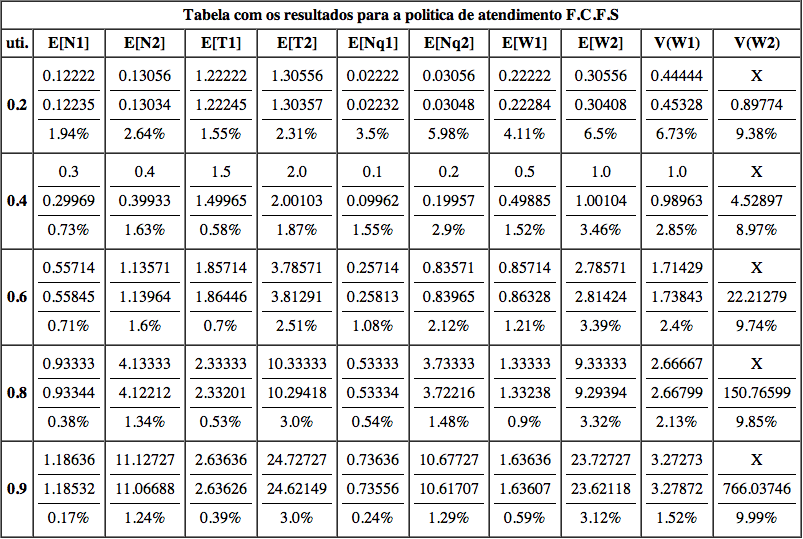
\includegraphics[width=1.0\textwidth]{tabelaFCFS.png}
   \caption{Tabela com os valores para a política de atendimento First Come First Served.}
\end{figure}
\label{fig:tabfcfs}

\pagebreak
\begin{figure}[htb!]
   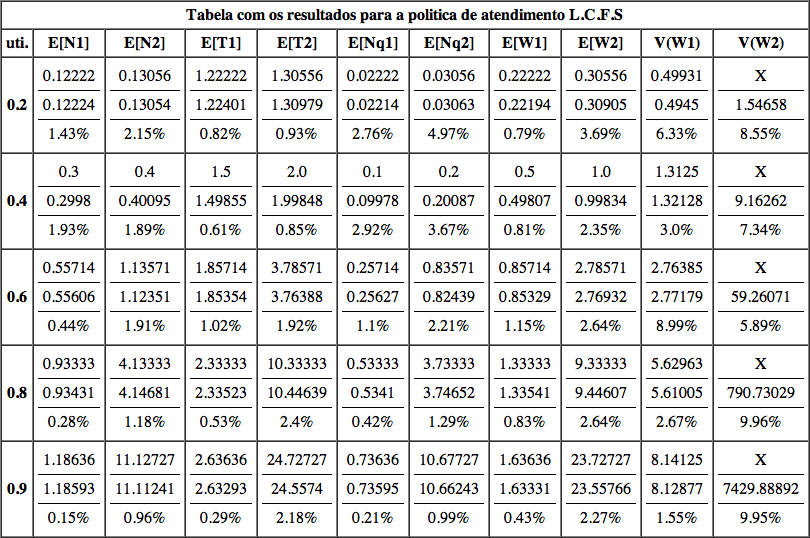
\includegraphics[width=1.0\textwidth]{tabelaLCFS.png}
   \caption{Tabela com os valores para a política de atendimento Last Come First Served.}
\end{figure}
\label{fig:tablcfs}

\pagebreak

O número de clientes avaliados em cada valor de utilização é explicitado na seção \ref{sec:parametros}.\\

O número de rodadas e tamanho da fase transiente para cada tipo de experimento é mostrado abaixo (os tamanho das fases transientes também são mostrados no capítulo \ref{chap:estimativa}, mas são expostos aqui também para facilidade de leitura):

\begin{itemize}
  \item $\rho=0.2$ - F.C.F.S : 5 rodadas - 30.000 clientes na fase transiente.
  \item $\rho=0.2$ - L.C.F.S : 4 rodadas - 30.000 clientes na fase transiente.
  \item $\rho=0.4$ - F.C.F.S : 11 rodadas - 40.000 clientes na fase transiente.
  \item $\rho=0.4$ - L.C.F.S : 5 rodadas - 40.000 clientes na fase transiente.
  \item $\rho=0.6$ - F.C.F.S : 14 rodadas - 80.000 clientes na fase transiente.
  \item $\rho=0.6$ - L.C.F.S : 4 rodadas - 80.000 clientes na fase transiente.
  \item $\rho=0.8$ - F.C.F.S : 19 rodadas - 400.000 clientes na fase transiente.
  \item $\rho=0.8$ - L.C.F.S : 31 rodadas - 400.000 clientes na fase transiente.
  \item $\rho=0.9$ - F.C.F.S : 76 rodadas - 500.000 clientes na fase transiente.
  \item $\rho=0.9$ - L.C.F.S : 106 rodadas - 500.000 clientes na fase transiente.
\end{itemize}

Como pode ser visto nas tabelas com os resultados, todos os valores analíticos se encontram dentro do intervalo de confiança estipulado pelo simulador.

\section{Comentários}
\label{sec:coment}

O valor da variância do tempo de espera da fila 2 não pode ser verificado analiticamente, portanto não há como ter certeza se o seu valor real se encontra dentro do intervalo de confiança. Porém podemos afirmar que há uma probabilidade grande dele se encontrar dentro do intervalo pois todos os outros valores estimados para a fila 2 estão dentro dos  intervalos de confiança calculados.

Esse mesmo valor foi o que comumente mais demorou a convergir para o intervalo de confiança válido, como mostrado nas tabelas \ref{fig:tabfcfs} e 4.2. Por isso usamos ele como métrica para definir a fase transiente como está mostrado na seção \ref{chap:estimativa}.

Verificamos empiricamente que avaliar 100.000 clientes por rodada de simulação fez com que os casos mais triviais, como por exemplo valor de utilização 0,2 e política de atendimento F.C.F.S chegassem aos valores desejados em um número menor de rodadas; e que os casos mais críticos, como $\rho=0.9$ e política L.C.F.S, convergissem ao resultado de maneira adequada.

Ao executar o simulador, para os diversos casos, verificamos o fato de que mesmo com o acréscimo de rodadas, o intervalo de confiança pode aumentar. Fato este que é explicado em que certas rodadas podem gerar médias relativamente distantes umas das outras, aumentando assim o desvio padrão numa taxa maior que a raiz quadrada do número de amostras. Nos resultados isso pôde ser verificado nos casos $\rho=0.4$ com política F.C.F.S e $\rho=0.6$ com política F.C.F.S, onde o número de rodadas necessário para se chegar a um resultado válido é bem maior do que casos bastante parecidos, como $\rho=0.4$ com política L.C.F.S.

Nos casos onde o valor de utilização se aproxima do limite para o sistema entrar em gargalo($\rho=0.8$ e $\rho=0.9$), o valor das variâncias encontradas diferem significativamente entre as duas políticas de atendimento usadas. No caso da fila 2, a variância para a política L.C.F.S chega a ser aproximadamente 10 vezes maior que a variância para a política F.C.F.S, em ambos os valores de utilização.

O caso mais crítico que foi avaliado ($\rho=0.9$ e política L.C.F.S), requeriu um tempo muito maior para convergir ao resultado do que os demais casos, acreditamos que isso se deve a seu valor de utilização estar bem próximo do valor em que o sistema entra em gargalo, e que a variância da fila 2 é de uma ordem de grandeza muito maior que todos os demais valores calculados, portanto demora mais para convergir o seu intervalo de confiança a um resultado válido.
